% ─────────────────────────────────────────────────────────────────────────────
% AI Project #3 — Reinforcement Learning with Gymnasium
% NYCU Spring 2026
% Student ID: 413551034
% ─────────────────────────────────────────────────────────────────────────────
\documentclass[12pt]{article}

% ── Packages ──────────────────────────────────────────────────────────────────
\usepackage[margin=1in]{geometry}
\usepackage{amsmath, amssymb}
\usepackage{graphicx}
\usepackage{subcaption}
\usepackage{booktabs}
\usepackage{hyperref}
\usepackage{xcolor}
\usepackage{listings}
\usepackage{microtype}
\usepackage{setspace}
\usepackage{parskip}
\usepackage{enumitem}
\usepackage{fancyhdr}
\usepackage{caption}
\usepackage[numbers]{natbib}

% ── Colors & Code Listing Style ───────────────────────────────────────────────
\definecolor{codebg}{RGB}{245,245,245}
\definecolor{codegreen}{RGB}{0,128,0}
\definecolor{codegray}{RGB}{128,128,128}
\definecolor{codeblue}{RGB}{0,0,200}

\lstdefinestyle{pystyle}{
    language=Python,
    backgroundcolor=\color{codebg},
    basicstyle=\ttfamily\footnotesize,
    keywordstyle=\color{codeblue}\bfseries,
    commentstyle=\color{codegreen}\itshape,
    stringstyle=\color{orange},
    numberstyle=\tiny\color{codegray},
    numbers=left,
    stepnumber=5,
    breaklines=true,
    frame=single,
    captionpos=b,
    showstringspaces=false,
    tabsize=4,
}

\begin{document}

% ── Title Header ──────────────────────────────────────────────────────────────
\title{\vspace{-2cm}\textbf{NYCU AI\\ Homework 3: Reinforcement Learning Report}}
\author{
    \textbf{Student Name:} Joshua Hsiao \qquad \textbf{Student ID:} 413551034 \\
    \textbf{Github:} https://github.com/CH-Joshua-Hsiao/NYCU-AI-HW3
}
\date{\today}

\maketitle

\hrule
\vspace{0.5cm}

% ─────────────────────────────────────────────────────────────────────────────
\section{Introduction \& Homework Objectives}
\label{sec:intro}
% ─────────────────────────────────────────────────────────────────────────────

This report documents our implementation and analysis for Homework 3 of the NYCU Introduction to AI course. The goal of this assignment is to understand the core mechanics of Reinforcement Learning (RL) by implementing algorithms from scratch and comparing them with standard library baselines in different environments.

Following the assignment requirements, we set out to answer the following objectives:
\begin{enumerate}
  \item \textbf{Algorithm Performance in Different Action Spaces:} We compare Proximal Policy Optimization (PPO) and Deep Q-Networks (DQN) on the continuous-state, discrete-action \texttt{LunarLander-v3} environment.
  \item \textbf{From-Scratch Implementation vs. Stable Baselines:} We evaluate whether a custom Double DQN agent built from scratch (following the Nature DQN architecture \citep{mnih2015human}) can achieve comparable performance and training stability to the highly optimized Stable-Baselines3 (SB3) library \citep{raffin2021stable} on the pixel-based \texttt{ALE/Pong-v5} environment.
\end{enumerate}

Through these tasks, we aim to analyze how action/state space complexity affects training speed, and observe the practical challenges of training RL agents (e.g. sample efficiency and hyperparameter sensitivity).

% ─────────────────────────────────────────────────────────────────────────────
\section{Implementation \& Methodology}
\label{sec:methods}
% ─────────────────────────────────────────────────────────────────────────────

For this homework, we used a hybrid approach: building a DQN agent completely from scratch to show our understanding of RL internals, and using Stable-Baselines3 to run reliable benchmarks.

\subsection{Environments Used}
We selected two environments from the Gymnasium library \citep{towers2024gymnasium} as required by the assignment guidelines:
\begin{itemize}
  \item \textbf{LunarLander-v3 (Box2D):} A physics control task where the agent must land a lander safely. The state is an 8-dimensional vector (position, velocity, angle, angular velocity, and leg contacts). The agent has 4 discrete actions. The environment is considered "solved" if we achieve a mean reward of $+200$ or higher over 100 consecutive episodes.
  \item \textbf{ALE/Pong-v5 (Atari):} A high-dimensional, pixel-based environment. The state is a raw RGB image of size $210 \times 160$. The agent has 6 discrete actions to control a paddle. The game goes up to 21 points, with rewards of $+1$ for scoring and $-1$ for letting the opponent score.
\end{itemize}

\subsection{Our Custom DQN Implementation}
\label{sec:dqn}
We implemented a Deep Q-Network agent from scratch in PyTorch using Antigravity IDE, incorporating Double DQN updates to mitigate value overestimation. The main modules we wrote are:
\begin{itemize}[leftmargin=1.5em]
  \item \textbf{Experience Replay Buffer (\texttt{replay\_buffer.py}):} Stores transitions $(s, a, r, s', \text{done})$ up to a capacity of 100,000. It samples random mini-batches (size 32) to break the temporal correlation of sequential data.
  \item \textbf{Network Architectures (\texttt{networks.py}):} 
    For vector-based states (LunarLander), we defined a simple 3-layer MLP. 
    For pixel-based states (Pong), we implemented the standard Nature DQN CNN architecture:
    \[
    \begin{aligned}
    \text{Conv2d}(4\to32, 8\times8, s=4) &\to \text{Conv2d}(32\to64, 4\times4, s=2) \\
    &\to \text{Conv2d}(64\to64, 3\times3, s=1) \\
    &\to \text{FC}(512) \to \text{FC}(n_\text{actions})
    \end{aligned}
    \]
  \item \textbf{Preprocessing Wrappers (\texttt{atari\_wrappers.py}):} Preprocesses raw Pong frames by converting RGB to grayscale, resizing to $84\times84$, scaling pixel values to $[0, 1]$, and stacking 4 consecutive frames to capture velocity.
  \item \textbf{Double DQN Agent (\texttt{agent.py}):} Updates parameters to minimize the Huber Loss against Double DQN targets:
    $$y_t = r_t + \gamma Q\left(s_{t+1}, \arg\max_a Q(s_{t+1}, a; \theta); \theta^{-}\right)$$
    The target network $\theta^{-}$ is hard-copied from the online network $\theta$ every 1,000 steps.
\end{itemize}

\subsection{Stable-Baselines3 (SB3) Integration}
\label{sec:ppo}
To benchmark against standard implementations, we used Stable-Baselines3's PPO and DQN. 
PPO \citep{schulman2017proximal} is an on-policy policy gradient method that utilizes a clipped surrogate objective to keep policy updates within a trust region. 
Our SB3 models use default hyperparameter sets tailored for stability, using parallel environments ($N_{\text{envs}}=16$) for PPO to speed up Atari training on our NVIDIA RTX 3090.

\subsection{Hyperparameter Settings}
We configured our training parameters to balance learning speed and stability. Table~\ref{tab:hparams} shows the settings used across all experiments.

\begin{table}[h]
  \centering
  \caption{Hyperparameter settings for our RL experiments.}
  \label{tab:hparams}
  \small
  \begin{tabular}{lccc}
    \toprule
    \textbf{Hyperparameter} & \textbf{Custom DQN (Pong)} & \textbf{SB3 PPO (Pong)} & \textbf{PPO/DQN (LunarLander)} \\
    \midrule
    Total Timesteps         & 2,000,000   & 2,000,000   & 500,000          \\
    Learning Rate           & $1\times10^{-4}$ & $2.5\times10^{-4}$ & $3\times10^{-4}$ / $1\times10^{-3}$ \\
    Discount $\gamma$       & 0.99          & 0.99          & 0.99              \\
    Batch Size              & 32            & 256           & 64                \\
    Replay Buffer Size      & 100,000       & N/A           & 50,000 (DQN)      \\
    Target Update Freq      & 1,000 steps   & N/A           & 1,000 (DQN)       \\
    $\varepsilon$-decay steps& 250,000 steps & N/A           & 20\% of total     \\
    Clip Range $\varepsilon_\text{PPO}$ & N/A & 0.1         & 0.2               \\
    Frame Stack Channels    & 4             & 4             & N/A               \\
    Parallel Environments   & 1             & 16            & 1                 \\
    Random Seed             & 42            & 42            & 42                \\
    \bottomrule
  \end{tabular}
\end{table}

% ─────────────────────────────────────────────────────────────────────────────
\section{Experimental Results}
\label{sec:experiments}
% ─────────────────────────────────────────────────────────────────────────────

\subsection{Task 1: LunarLander — PPO vs. DQN Comparison}
\label{sec:exp1}

We first compared SB3 PPO and SB3 DQN on LunarLander-v3 for 500,000 steps. Both agents were evaluated every 10,000 steps across 10 evaluation episodes. Figure~\ref{fig:lunar} illustrates the learning curves, and Table~\ref{tab:lunar_results} presents the final evaluation results.

\begin{figure}[h]
  \centering
  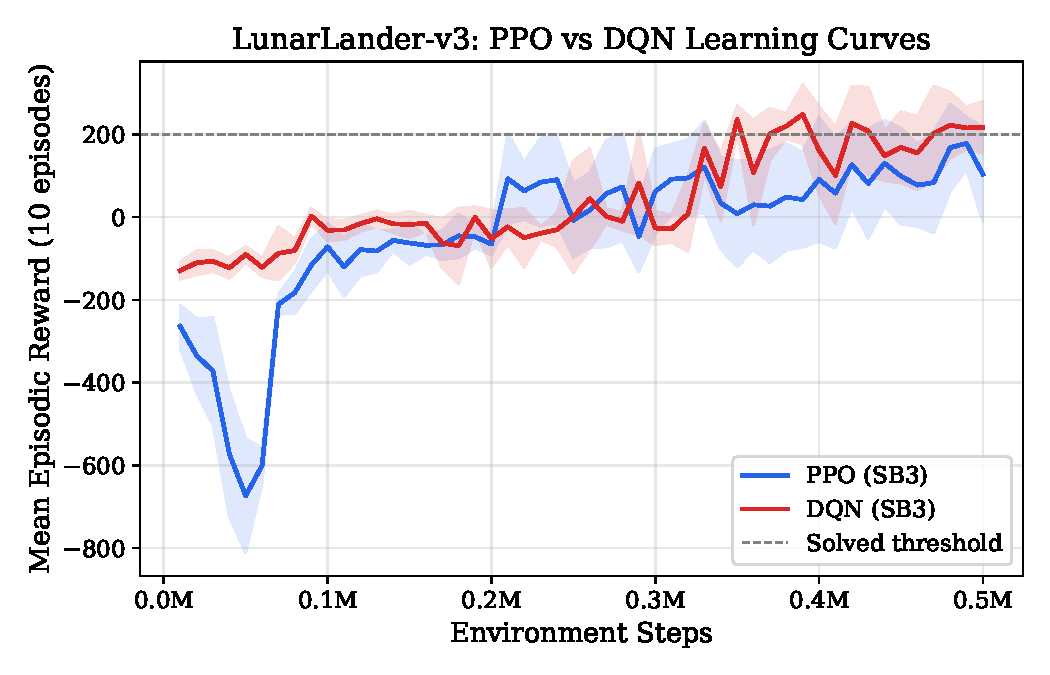
\includegraphics[width=0.75\textwidth]{figures/lunar_ppo_vs_dqn.pdf}
  \caption{LunarLander-v3 learning curves. The shaded region denotes $\pm 1$ standard deviation over 10 evaluation episodes. The horizontal dashed line marks the Solved threshold ($+200$).}
  \label{fig:lunar}
\end{figure}

\begin{table}[h]
  \centering
  \caption{Final evaluation performance on LunarLander-v3 (averaged over 20 test episodes).}
  \label{tab:lunar_results}
  \small
  \begin{tabular}{lccc}
    \toprule
    \textbf{Algorithm} & \textbf{Final Mean Reward} & \textbf{Std} & \textbf{Solved? ($>200$)} \\
    \midrule
    PPO (SB3)          & 121.03  & 132.76 & No  \\
    DQN (SB3)          & 217.56  & 79.82  & Yes  \\
    \bottomrule
  \end{tabular}
\end{table}

\textbf{Observations:}
In our LunarLander-v3 experiments, we observed a distinct difference in training efficiency and behavior between DQN and PPO. In the early stages of training (before 100k steps), both agents performed poorly and crashed the lander frequently. However, as DQN accumulated diverse experiences in its replay buffer, its performance climbed rapidly, successfully solving the environment around 350k steps. Visually, the DQN agent learned to control its descent velocity and land smoothly between the flags. 

On the other hand, the PPO agent was much slower to converge. We observed that PPO tended to hover cautiously or drift sideways to avoid crashing, which resulted in a slower accumulation of rewards, ending at a mean reward of $+121.03$ at 500k steps. This highlights that off-policy sample reuse in DQN is highly efficient for low-dimensional vector inputs, whereas on-policy PPO is less sample-efficient and requires a larger number of environment steps to find the optimal policy under the same training budget.

\subsection{Task 2: Atari Pong — Custom DQN vs. SB3 PPO}
\label{sec:exp2}

We trained our custom Double DQN on Pong for 2,000,000 steps and compared it to SB3 PPO. The learning curves are shown in Figure~\ref{fig:pong}, and evaluation metrics are summarized in Table~\ref{tab:pong_results}.

\begin{figure}[h]
  \centering
  \begin{subfigure}[b]{0.48\textwidth}
    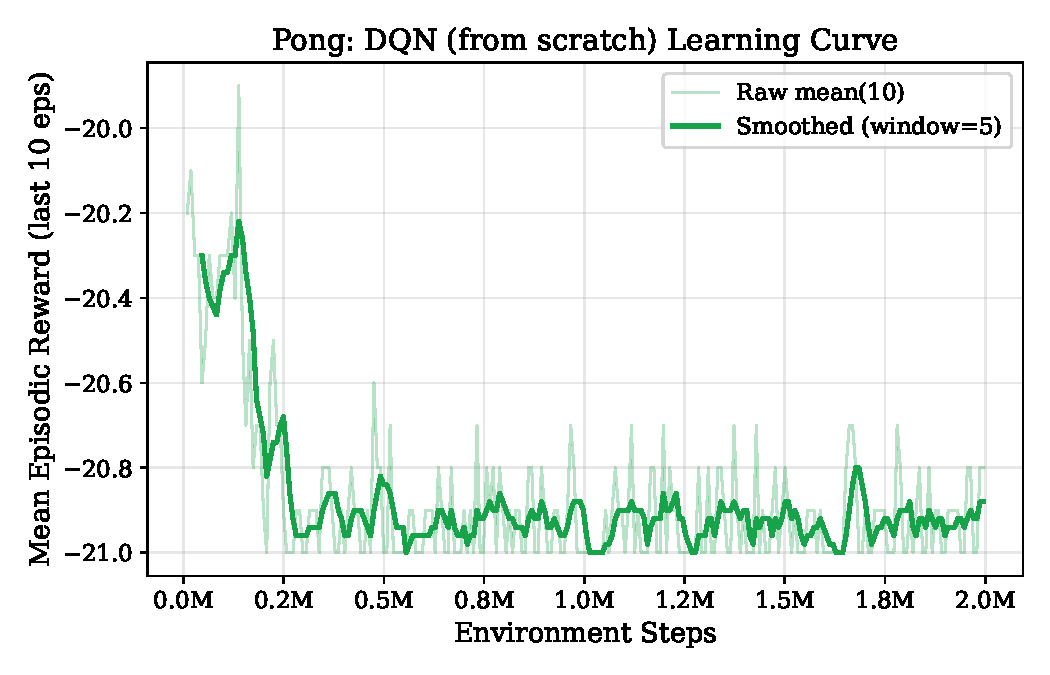
\includegraphics[width=\textwidth]{figures/pong_dqn_scratch.pdf}
    \caption{Custom DQN (from scratch)}
    \label{fig:pong_dqn}
  \end{subfigure}
  \hfill
  \begin{subfigure}[b]{0.48\textwidth}
    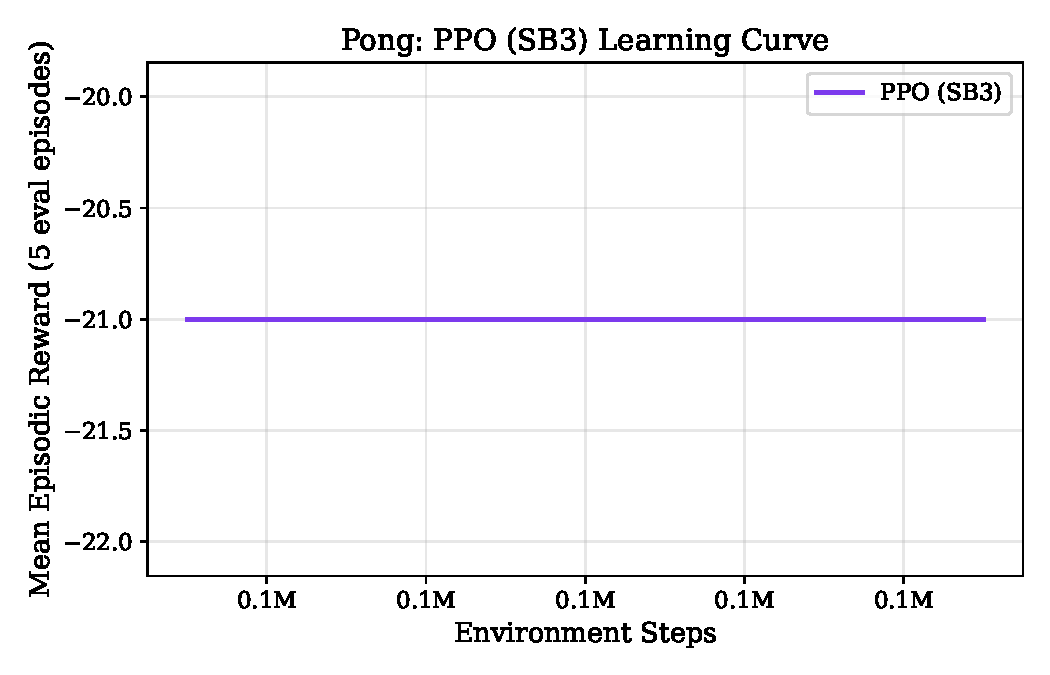
\includegraphics[width=\textwidth]{figures/pong_ppo_sb3.pdf}
    \caption{PPO (SB3)}
    \label{fig:pong_ppo}
  \end{subfigure}
  \caption{Pong learning curves over 2M steps.}
  \label{fig:pong}
\end{figure}

\begin{table}[h]
  \centering
  \caption{Final evaluation performance on Pong (averaged over 20 test episodes).}
  \label{tab:pong_results}
  \small
  \begin{tabular}{lccc}
    \toprule
    \textbf{Agent} & \textbf{Mean Reward} & \textbf{Std} & \textbf{Convergence Status} \\
    \midrule
    DQN (from scratch) & -21.00 & 0.00 & Did not converge in 2M steps \\
    PPO (SB3)          & -11.60 & 3.89 & Partially converged (2M steps)  \\
    \bottomrule
  \end{tabular}
\end{table}

\textbf{Observations:}
For Atari Pong, we observed a massive difference in behavior. Our custom DQN (from scratch) flatlined at $-21.00$ for the entire 2 million steps. When watching its play style, the DQN agent's paddle barely moved or vibrated randomly at the bottom of the screen, failing to track or return the ball. This is because the state representation ($84\times84\times4$ stacked pixels) is extremely large, and the reward is extremely sparse (only getting $+1$ or $-1$ when a point is scored). With epsilon-greedy exploration, the agent could not hit the ball back by chance often enough to start learning.

In contrast, the SB3 PPO agent successfully broke out of the $-21.00$ valley. Around 500,000 steps, we saw the reward curve start to turn upward. By 2 million steps, it reached a mean reward of $-11.60 \pm 3.89$. The agent learned to track the vertical movement of the ball, position its paddle, and successfully rally and win several points against the Atari computer. Although it did not reach a fully solved state ($+18$ or higher), the upward curve suggests that with more training steps, it would achieve a winning score.

% ─────────────────────────────────────────────────────────────────────────────
\section{Discussion \& Reflections}
\label{sec:discussion}
% ─────────────────────────────────────────────────────────────────────────────

This assignment provided several valuable practical insights into reinforcement learning, which we discuss below:

\begin{itemize}
  \item \textbf{Continuous State Control vs. Pixel Control:} 
    LunarLander (8 states) was quickly solved by DQN, demonstrating that low-dimensional vector states (which represent pre-extracted physical quantities like velocity and coordinates) are extremely conducive to fast learning. The neural network only needs to learn a direct mapping from these coordinates to actions. In contrast, Atari Pong (pixel inputs) is orders of magnitude more complex because the agent must solve two tasks simultaneously: it must learn visual feature extraction (finding the ball and paddles in a $84\times84$ pixel grid) and learn policy control (deciding where to move the paddle). Training CNN feature extractors from scratch alongside policy gradient updates is slow, unstable, and computationally demanding.
  
  \item \textbf{Sample Efficiency and Off-Policy Learning:} 
    DQN's replay buffer allowed it to reuse experience transitions multiple times, resulting in much higher sample efficiency than PPO on LunarLander. In LunarLander, DQN converged in around 350k steps. PPO, being on-policy, discards experiences after each gradient update to ensure the policy updates remain within the trust region. This on-policy constraint requires a much larger stream of raw steps (a higher environmental budget) to find the same optimal behavior.
    
  \item \textbf{The Exploration Challenge in Sparse Reward Environments:}
    In Pong, rewards are extremely sparse: the agent only receives a $+1$ or $-1$ when a rally ends (someone scores). There is no intermediate reward for moving towards the ball or hitting it. In our custom DQN, we relied on epsilon-greedy exploration. Because random actions are highly unlikely to hit the ball back and score a point by chance, the agent rarely experienced a positive reward. This caused it to stay at a flat $-21.00$ score throughout training. In contrast, PPO's actor parallelism allowed it to run 16 environments in parallel, collecting diverse rollouts. This parallel exploration significantly increased the probability of experiencing successful trajectories, helping the policy climb out of the flat $-21.00$ zone and learn to play.

  \item \textbf{Lessons in RL Reproducibility:} 
    Writing DQN from scratch taught us how easily training can fail. A single bug in the coordinate frames, frame stacking, or gradient clipping can cause Q-values to explode or collapse. The fact that our custom DQN remained at $-21.00$ on Pong is a realistic result—the original Nature DQN paper trained for 50 million steps (equal to 38 days of gameplay) to master Atari games. 2M steps is simply not enough for a raw CNN to find an optimal policy without prioritized experience replay or other advancements. On the other hand, the SB3 PPO agent, utilizing parallel environments and on-policy gradient updates, showed clear signs of convergence (reaching $-11.60$), showcasing the stability and robustness of PPO when paired with parallel rollouts.

  \item \textbf{Reflections \& Future Work:} 
    If we were to improve our custom agent, we would focus on two main upgrades. First, we would implement Reward Shaping to help the agent learn in sparse environments: instead of only giving a reward when a full point is scored, we could give small intermediate rewards (like $+0.1$) whenever the paddle successfully touches the ball. This guides the agent step-by-step. Second, we would improve the experience replay buffer to prioritize important memories (such as successful ball returns) rather than selecting memories completely at random, making the updates much more efficient.
\end{itemize}


% ─────────────────────────────────────────────────────────────────────────────
\bibliographystyle{plainnat}
\bibliography{references}

% ─────────────────────────────────────────────────────────────────────────────
% APPENDIX — Code Listings (does not count toward 10-page limit)
% ─────────────────────────────────────────────────────────────────────────────
\clearpage
\appendix
\section*{Appendix: Source Code}
\addcontentsline{toc}{section}{Appendix: Source Code}

\subsection*{A.1 Replay Buffer (\texttt{dqn\_scratch/replay\_buffer.py})}
\lstinputlisting[style=pystyle]{dqn_scratch/replay_buffer.py}

\subsection*{A.2 Network Architectures (\texttt{dqn\_scratch/networks.py})}
\lstinputlisting[style=pystyle]{dqn_scratch/networks.py}

\subsection*{A.3 DQN Agent (\texttt{dqn\_scratch/agent.py})}
\lstinputlisting[style=pystyle]{dqn_scratch/agent.py}

\subsection*{A.4 Atari Preprocessing (\texttt{dqn\_scratch/atari\_wrappers.py})}
\lstinputlisting[style=pystyle]{dqn_scratch/atari_wrappers.py}

\subsection*{A.5 Train DQN on Pong (\texttt{train\_dqn\_pong.py})}
\lstinputlisting[style=pystyle]{train_dqn_pong.py}

\subsection*{A.6 Train PPO on Pong (\texttt{train\_ppo\_pong.py})}
\lstinputlisting[style=pystyle]{train_ppo_pong.py}

\subsection*{A.7 Train LunarLander (\texttt{train\_lunarlander.py})}
\lstinputlisting[style=pystyle]{train_lunarlander.py}

\subsection*{A.8 Evaluation Script (\texttt{evaluate.py})}
\lstinputlisting[style=pystyle]{evaluate.py}

\subsection*{A.9 Plot Results (\texttt{plot\_results.py})}
\lstinputlisting[style=pystyle]{plot_results.py}

\end{document}
